\documentclass[twoside]{book}

% Packages required by doxygen
\usepackage{fixltx2e}
\usepackage{calc}
\usepackage{doxygen}
\usepackage{graphicx}
\usepackage[utf8]{inputenc}
\usepackage{makeidx}
\usepackage{multicol}
\usepackage{multirow}
\PassOptionsToPackage{warn}{textcomp}
\usepackage{textcomp}
\usepackage[nointegrals]{wasysym}
\usepackage[table]{xcolor}

% Font selection
\usepackage[T1]{fontenc}
\usepackage{mathptmx}
\usepackage[scaled=.90]{helvet}
\usepackage{courier}
\usepackage{amssymb}
\usepackage{sectsty}
\renewcommand{\familydefault}{\sfdefault}
\allsectionsfont{%
  \fontseries{bc}\selectfont%
  \color{darkgray}%
}
\renewcommand{\DoxyLabelFont}{%
  \fontseries{bc}\selectfont%
  \color{darkgray}%
}
\newcommand{\+}{\discretionary{\mbox{\scriptsize$\hookleftarrow$}}{}{}}

% Page & text layout
\usepackage{geometry}
\geometry{%
  a4paper,%
  top=2.5cm,%
  bottom=2.5cm,%
  left=2.5cm,%
  right=2.5cm%
}
\tolerance=750
\hfuzz=15pt
\hbadness=750
\setlength{\emergencystretch}{15pt}
\setlength{\parindent}{0cm}
\setlength{\parskip}{0.2cm}
\makeatletter
\renewcommand{\paragraph}{%
  \@startsection{paragraph}{4}{0ex}{-1.0ex}{1.0ex}{%
    \normalfont\normalsize\bfseries\SS@parafont%
  }%
}
\renewcommand{\subparagraph}{%
  \@startsection{subparagraph}{5}{0ex}{-1.0ex}{1.0ex}{%
    \normalfont\normalsize\bfseries\SS@subparafont%
  }%
}
\makeatother

% Headers & footers
\usepackage{fancyhdr}
\pagestyle{fancyplain}
\fancyhead[LE]{\fancyplain{}{\bfseries\thepage}}
\fancyhead[CE]{\fancyplain{}{}}
\fancyhead[RE]{\fancyplain{}{\bfseries\leftmark}}
\fancyhead[LO]{\fancyplain{}{\bfseries\rightmark}}
\fancyhead[CO]{\fancyplain{}{}}
\fancyhead[RO]{\fancyplain{}{\bfseries\thepage}}
\fancyfoot[LE]{\fancyplain{}{}}
\fancyfoot[CE]{\fancyplain{}{}}
\fancyfoot[RE]{\fancyplain{}{\bfseries\scriptsize Generated on Thu Feb 1 2018 18\+:39\+:42 for Neuro\+Wood by Doxygen }}
\fancyfoot[LO]{\fancyplain{}{\bfseries\scriptsize Generated on Thu Feb 1 2018 18\+:39\+:42 for Neuro\+Wood by Doxygen }}
\fancyfoot[CO]{\fancyplain{}{}}
\fancyfoot[RO]{\fancyplain{}{}}
\renewcommand{\footrulewidth}{0.4pt}
\renewcommand{\chaptermark}[1]{%
  \markboth{#1}{}%
}
\renewcommand{\sectionmark}[1]{%
  \markright{\thesection\ #1}%
}

% Indices & bibliography
\usepackage{natbib}
\usepackage[titles]{tocloft}
\setcounter{tocdepth}{3}
\setcounter{secnumdepth}{5}
\makeindex

% Hyperlinks (required, but should be loaded last)
\usepackage{ifpdf}
\ifpdf
  \usepackage[pdftex,pagebackref=true]{hyperref}
\else
  \usepackage[ps2pdf,pagebackref=true]{hyperref}
\fi
\hypersetup{%
  colorlinks=true,%
  linkcolor=blue,%
  citecolor=blue,%
  unicode%
}

% Custom commands
\newcommand{\clearemptydoublepage}{%
  \newpage{\pagestyle{empty}\cleardoublepage}%
}


%===== C O N T E N T S =====

\begin{document}

% Titlepage & ToC
\hypersetup{pageanchor=false,
             bookmarks=true,
             bookmarksnumbered=true,
             pdfencoding=unicode
            }
\pagenumbering{roman}
\begin{titlepage}
\vspace*{7cm}
\begin{center}%
{\Large Neuro\+Wood \\[1ex]\large 0.\+0.\+2 }\\
\vspace*{1cm}
{\large Generated by Doxygen 1.8.7}\\
\vspace*{0.5cm}
{\small Thu Feb 1 2018 18:39:42}\\
\end{center}
\end{titlepage}
\clearemptydoublepage
\tableofcontents
\clearemptydoublepage
\pagenumbering{arabic}
\hypersetup{pageanchor=true}

%--- Begin generated contents ---
\chapter{neurowood}
\label{md__r_e_a_d_m_e}
\hypertarget{md__r_e_a_d_m_e}{}
\input{md__r_e_a_d_m_e}
\chapter{Hierarchical Index}
\section{Class Hierarchy}
This inheritance list is sorted roughly, but not completely, alphabetically\+:\begin{DoxyCompactList}
\item \contentsline{section}{Classifier}{\pageref{class_classifier}}{}
\item \contentsline{section}{Classifier\+\_\+builder}{\pageref{class_classifier__builder}}{}
\item \contentsline{section}{E\+X\+T\+R\+A\+C\+T\+O\+R\+\_\+\+D\+A\+T\+A}{\pageref{struct_e_x_t_r_a_c_t_o_r___d_a_t_a}}{}
\item \contentsline{section}{E\+X\+T\+R\+A\+C\+T\+O\+R\+\_\+\+P\+A\+R\+A\+M\+S}{\pageref{struct_e_x_t_r_a_c_t_o_r___p_a_r_a_m_s}}{}
\begin{DoxyCompactList}
\item \contentsline{section}{H\+A\+R\+A\+L\+I\+C\+K\+\_\+\+P\+A\+R\+A\+M\+S}{\pageref{struct_h_a_r_a_l_i_c_k___p_a_r_a_m_s}}{}
\item \contentsline{section}{L\+B\+P\+\_\+\+P\+A\+R\+A\+M\+S}{\pageref{struct_l_b_p___p_a_r_a_m_s}}{}
\end{DoxyCompactList}
\item \contentsline{section}{Ftr\+\_\+extractor}{\pageref{class_ftr__extractor}}{}
\begin{DoxyCompactList}
\item \contentsline{section}{Haralick\+\_\+extractor}{\pageref{class_haralick__extractor}}{}
\item \contentsline{section}{L\+B\+P\+\_\+extractor}{\pageref{class_l_b_p__extractor}}{}
\end{DoxyCompactList}
\item \contentsline{section}{Im\+\_\+processing}{\pageref{class_im__processing}}{}
\begin{DoxyCompactList}
\item \contentsline{section}{Color\+\_\+filter}{\pageref{class_color__filter}}{}
\item \contentsline{section}{Crop\+\_\+image}{\pageref{class_crop__image}}{}
\item \contentsline{section}{Noise\+\_\+filter}{\pageref{class_noise__filter}}{}
\end{DoxyCompactList}
\item \contentsline{section}{I\+M\+P\+R\+O\+C\+\_\+\+D\+A\+T\+A}{\pageref{struct_i_m_p_r_o_c___d_a_t_a}}{}
\item \contentsline{section}{I\+M\+P\+R\+O\+C\+\_\+\+P\+A\+R\+A\+M\+S}{\pageref{struct_i_m_p_r_o_c___p_a_r_a_m_s}}{}
\begin{DoxyCompactList}
\item \contentsline{section}{C\+O\+L\+O\+R\+\_\+\+P\+A\+R\+A\+M\+S}{\pageref{struct_c_o_l_o_r___p_a_r_a_m_s}}{}
\item \contentsline{section}{C\+R\+O\+P\+\_\+\+P\+A\+R\+A\+M\+S}{\pageref{struct_c_r_o_p___p_a_r_a_m_s}}{}
\item \contentsline{section}{N\+O\+I\+S\+E\+\_\+\+P\+A\+R\+A\+M\+S}{\pageref{struct_n_o_i_s_e___p_a_r_a_m_s}}{}
\end{DoxyCompactList}
\item \contentsline{section}{Model}{\pageref{class_model}}{}
\begin{DoxyCompactList}
\item \contentsline{section}{K\+N\+N\+\_\+\+Model}{\pageref{class_k_n_n___model}}{}
\item \contentsline{section}{M\+L\+P\+\_\+\+Model}{\pageref{class_m_l_p___model}}{}
\end{DoxyCompactList}
\item \contentsline{section}{Model\+\_\+trainer}{\pageref{class_model__trainer}}{}
\begin{DoxyCompactList}
\item \contentsline{section}{K\+N\+N\+\_\+trainer}{\pageref{class_k_n_n__trainer}}{}
\item \contentsline{section}{M\+L\+P\+\_\+trainer}{\pageref{class_m_l_p__trainer}}{}
\end{DoxyCompactList}
\end{DoxyCompactList}

\chapter{Class Index}
\section{Class List}
Here are the classes, structs, unions and interfaces with brief descriptions\+:\begin{DoxyCompactList}
\item\contentsline{section}{\hyperlink{class_classifier}{Classifier} }{\pageref{class_classifier}}{}
\item\contentsline{section}{\hyperlink{class_classifier__builder}{Classifier\+\_\+builder} }{\pageref{class_classifier__builder}}{}
\item\contentsline{section}{\hyperlink{class_color__filter}{Color\+\_\+filter} }{\pageref{class_color__filter}}{}
\item\contentsline{section}{\hyperlink{struct_c_o_l_o_r___p_a_r_a_m_s}{C\+O\+L\+O\+R\+\_\+\+P\+A\+R\+A\+M\+S} }{\pageref{struct_c_o_l_o_r___p_a_r_a_m_s}}{}
\item\contentsline{section}{\hyperlink{class_crop__image}{Crop\+\_\+image} }{\pageref{class_crop__image}}{}
\item\contentsline{section}{\hyperlink{struct_c_r_o_p___p_a_r_a_m_s}{C\+R\+O\+P\+\_\+\+P\+A\+R\+A\+M\+S} }{\pageref{struct_c_r_o_p___p_a_r_a_m_s}}{}
\item\contentsline{section}{\hyperlink{struct_e_x_t_r_a_c_t_o_r___d_a_t_a}{E\+X\+T\+R\+A\+C\+T\+O\+R\+\_\+\+D\+A\+T\+A} }{\pageref{struct_e_x_t_r_a_c_t_o_r___d_a_t_a}}{}
\item\contentsline{section}{\hyperlink{struct_e_x_t_r_a_c_t_o_r___p_a_r_a_m_s}{E\+X\+T\+R\+A\+C\+T\+O\+R\+\_\+\+P\+A\+R\+A\+M\+S} }{\pageref{struct_e_x_t_r_a_c_t_o_r___p_a_r_a_m_s}}{}
\item\contentsline{section}{\hyperlink{class_ftr__extractor}{Ftr\+\_\+extractor} }{\pageref{class_ftr__extractor}}{}
\item\contentsline{section}{\hyperlink{class_haralick__extractor}{Haralick\+\_\+extractor} }{\pageref{class_haralick__extractor}}{}
\item\contentsline{section}{\hyperlink{struct_h_a_r_a_l_i_c_k___p_a_r_a_m_s}{H\+A\+R\+A\+L\+I\+C\+K\+\_\+\+P\+A\+R\+A\+M\+S} }{\pageref{struct_h_a_r_a_l_i_c_k___p_a_r_a_m_s}}{}
\item\contentsline{section}{\hyperlink{class_im__processing}{Im\+\_\+processing} }{\pageref{class_im__processing}}{}
\item\contentsline{section}{\hyperlink{struct_i_m_p_r_o_c___d_a_t_a}{I\+M\+P\+R\+O\+C\+\_\+\+D\+A\+T\+A} }{\pageref{struct_i_m_p_r_o_c___d_a_t_a}}{}
\item\contentsline{section}{\hyperlink{struct_i_m_p_r_o_c___p_a_r_a_m_s}{I\+M\+P\+R\+O\+C\+\_\+\+P\+A\+R\+A\+M\+S} }{\pageref{struct_i_m_p_r_o_c___p_a_r_a_m_s}}{}
\item\contentsline{section}{\hyperlink{class_k_n_n___model}{K\+N\+N\+\_\+\+Model} }{\pageref{class_k_n_n___model}}{}
\item\contentsline{section}{\hyperlink{class_k_n_n__trainer}{K\+N\+N\+\_\+trainer} }{\pageref{class_k_n_n__trainer}}{}
\item\contentsline{section}{\hyperlink{class_l_b_p__extractor}{L\+B\+P\+\_\+extractor} }{\pageref{class_l_b_p__extractor}}{}
\item\contentsline{section}{\hyperlink{struct_l_b_p___p_a_r_a_m_s}{L\+B\+P\+\_\+\+P\+A\+R\+A\+M\+S} }{\pageref{struct_l_b_p___p_a_r_a_m_s}}{}
\item\contentsline{section}{\hyperlink{class_m_l_p___model}{M\+L\+P\+\_\+\+Model} }{\pageref{class_m_l_p___model}}{}
\item\contentsline{section}{\hyperlink{class_m_l_p__trainer}{M\+L\+P\+\_\+trainer} }{\pageref{class_m_l_p__trainer}}{}
\item\contentsline{section}{\hyperlink{class_model}{Model} }{\pageref{class_model}}{}
\item\contentsline{section}{\hyperlink{class_model__trainer}{Model\+\_\+trainer} }{\pageref{class_model__trainer}}{}
\item\contentsline{section}{\hyperlink{class_noise__filter}{Noise\+\_\+filter} }{\pageref{class_noise__filter}}{}
\item\contentsline{section}{\hyperlink{struct_n_o_i_s_e___p_a_r_a_m_s}{N\+O\+I\+S\+E\+\_\+\+P\+A\+R\+A\+M\+S} }{\pageref{struct_n_o_i_s_e___p_a_r_a_m_s}}{}
\end{DoxyCompactList}

\chapter{Class Documentation}
\hypertarget{class_classifier}{\section{Classifier Class Reference}
\label{class_classifier}\index{Classifier@{Classifier}}
}
\subsection*{Public Member Functions}
\begin{DoxyCompactItemize}
\item 
\hypertarget{class_classifier_afd14ddf13364da1a9bd5b1e45eab9b3f}{int {\bfseries classify} (cv\+::\+Mat $\ast$input\+\_\+img)}\label{class_classifier_afd14ddf13364da1a9bd5b1e45eab9b3f}

\item 
\hypertarget{class_classifier_a472a413b30e86e522e2a7894416956cd}{void {\bfseries train} ()}\label{class_classifier_a472a413b30e86e522e2a7894416956cd}

\end{DoxyCompactItemize}


The documentation for this class was generated from the following file\+:\begin{DoxyCompactItemize}
\item 
Classifier.\+hpp\end{DoxyCompactItemize}

\hypertarget{class_classifier__builder}{\section{Classifier\+\_\+builder Class Reference}
\label{class_classifier__builder}\index{Classifier\+\_\+builder@{Classifier\+\_\+builder}}
}
\subsection*{Public Member Functions}
\begin{DoxyCompactItemize}
\item 
\hypertarget{class_classifier__builder_a9b6ef2588fe70aa48258b2f8f59d82f9}{\hyperlink{class_classifier}{Classifier} $\ast$ {\bfseries build\+\_\+classifier} (char $\ast$nome\+\_\+arquivo\+\_\+parametros)}\label{class_classifier__builder_a9b6ef2588fe70aa48258b2f8f59d82f9}

\item 
\hypertarget{class_classifier__builder_ad836ba2a05cc1ae0aaea279ff60fb0e7}{\hyperlink{class_im__processing}{Im\+\_\+processing} $\ast$ {\bfseries build\+\_\+img\+\_\+processing} (enum\+Im\+Processing tipo, Mat $\ast$params)}\label{class_classifier__builder_ad836ba2a05cc1ae0aaea279ff60fb0e7}

\item 
\hypertarget{class_classifier__builder_a45f684052b0a27dbb826bcab8265b32d}{\hyperlink{class_ftr__extractor}{Ftr\+\_\+extractor} $\ast$ {\bfseries build\+\_\+ftr\+\_\+extractor} (enum\+Descriptors tipo, Mat $\ast$params)}\label{class_classifier__builder_a45f684052b0a27dbb826bcab8265b32d}

\item 
\hypertarget{class_classifier__builder_a6080594fee5e01afe55d5c481c7a95ba}{\hyperlink{class_model}{Model} $\ast$ {\bfseries build\+\_\+model} (enum\+Models tipo, Mat $\ast$params)}\label{class_classifier__builder_a6080594fee5e01afe55d5c481c7a95ba}

\item 
\hypertarget{class_classifier__builder_a3efa3afcb9bdc6dc1a9771d82852120f}{\hyperlink{class_model__trainer}{Model\+\_\+trainer} $\ast$ {\bfseries build\+\_\+trainer} ()}\label{class_classifier__builder_a3efa3afcb9bdc6dc1a9771d82852120f}

\end{DoxyCompactItemize}


The documentation for this class was generated from the following files\+:\begin{DoxyCompactItemize}
\item 
Classifier\+\_\+builder.\+hpp\item 
Classifier\+\_\+builder.\+cpp\end{DoxyCompactItemize}

\hypertarget{class_color__filter}{\section{Color\+\_\+filter Class Reference}
\label{class_color__filter}\index{Color\+\_\+filter@{Color\+\_\+filter}}
}
Inheritance diagram for Color\+\_\+filter\+:\begin{figure}[H]
\begin{center}
\leavevmode
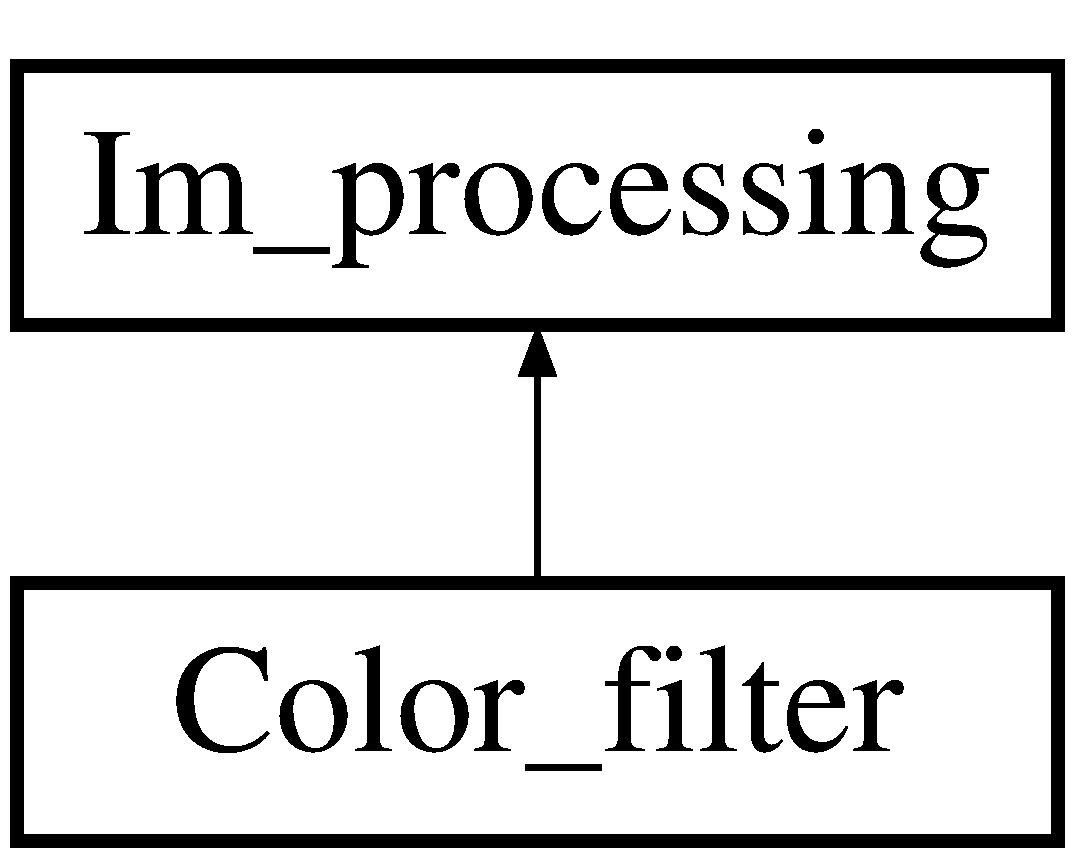
\includegraphics[height=2.000000cm]{class_color__filter}
\end{center}
\end{figure}
\subsection*{Public Member Functions}
\begin{DoxyCompactItemize}
\item 
\hypertarget{class_color__filter_a8cc00b7039652d79413886b762c2029a}{void {\bfseries apply} (int $\ast$n)}\label{class_color__filter_a8cc00b7039652d79413886b762c2029a}

\end{DoxyCompactItemize}


The documentation for this class was generated from the following files\+:\begin{DoxyCompactItemize}
\item 
Im\+\_\+processing.\+hpp\item 
Im\+\_\+processing.\+cpp\end{DoxyCompactItemize}

\hypertarget{struct_c_o_l_o_r___p_a_r_a_m_s}{\section{C\+O\+L\+O\+R\+\_\+\+P\+A\+R\+A\+M\+S Struct Reference}
\label{struct_c_o_l_o_r___p_a_r_a_m_s}\index{C\+O\+L\+O\+R\+\_\+\+P\+A\+R\+A\+M\+S@{C\+O\+L\+O\+R\+\_\+\+P\+A\+R\+A\+M\+S}}
}
Inheritance diagram for C\+O\+L\+O\+R\+\_\+\+P\+A\+R\+A\+M\+S\+:\begin{figure}[H]
\begin{center}
\leavevmode
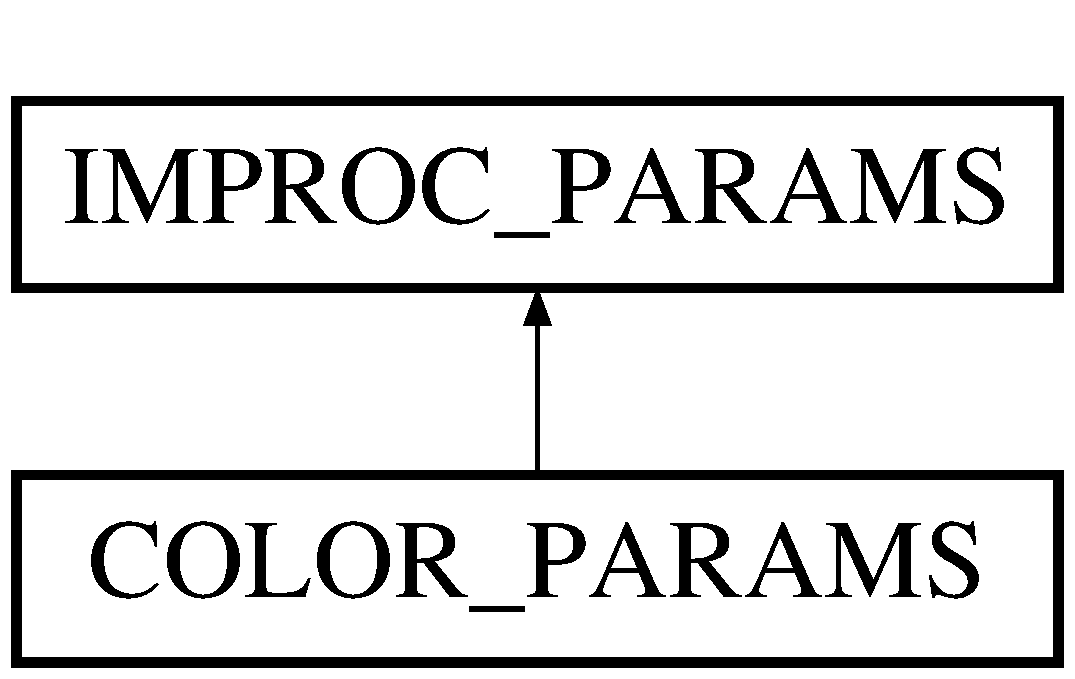
\includegraphics[height=2.000000cm]{struct_c_o_l_o_r___p_a_r_a_m_s}
\end{center}
\end{figure}


The documentation for this struct was generated from the following file\+:\begin{DoxyCompactItemize}
\item 
Im\+\_\+processing.\+hpp\end{DoxyCompactItemize}

\hypertarget{class_crop__image}{\section{Crop\+\_\+image Class Reference}
\label{class_crop__image}\index{Crop\+\_\+image@{Crop\+\_\+image}}
}
Inheritance diagram for Crop\+\_\+image\+:\begin{figure}[H]
\begin{center}
\leavevmode
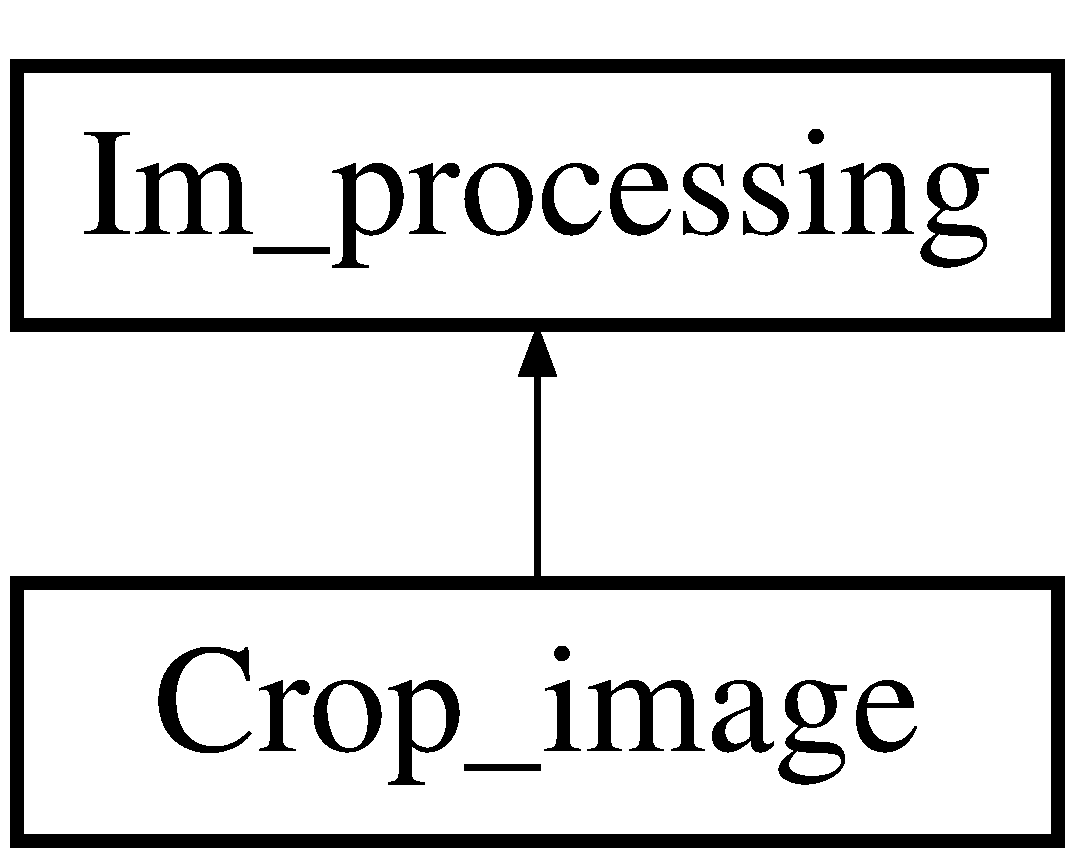
\includegraphics[height=2.000000cm]{class_crop__image}
\end{center}
\end{figure}
\subsection*{Public Member Functions}
\begin{DoxyCompactItemize}
\item 
\hypertarget{class_crop__image_afb126cc9f7a3c57ce94a0e483fe2d217}{void {\bfseries apply} (int $\ast$n)}\label{class_crop__image_afb126cc9f7a3c57ce94a0e483fe2d217}

\end{DoxyCompactItemize}


The documentation for this class was generated from the following files\+:\begin{DoxyCompactItemize}
\item 
Im\+\_\+processing.\+hpp\item 
Im\+\_\+processing.\+cpp\end{DoxyCompactItemize}

\hypertarget{struct_c_r_o_p___p_a_r_a_m_s}{\section{C\+R\+O\+P\+\_\+\+P\+A\+R\+A\+M\+S Struct Reference}
\label{struct_c_r_o_p___p_a_r_a_m_s}\index{C\+R\+O\+P\+\_\+\+P\+A\+R\+A\+M\+S@{C\+R\+O\+P\+\_\+\+P\+A\+R\+A\+M\+S}}
}
Inheritance diagram for C\+R\+O\+P\+\_\+\+P\+A\+R\+A\+M\+S\+:\begin{figure}[H]
\begin{center}
\leavevmode
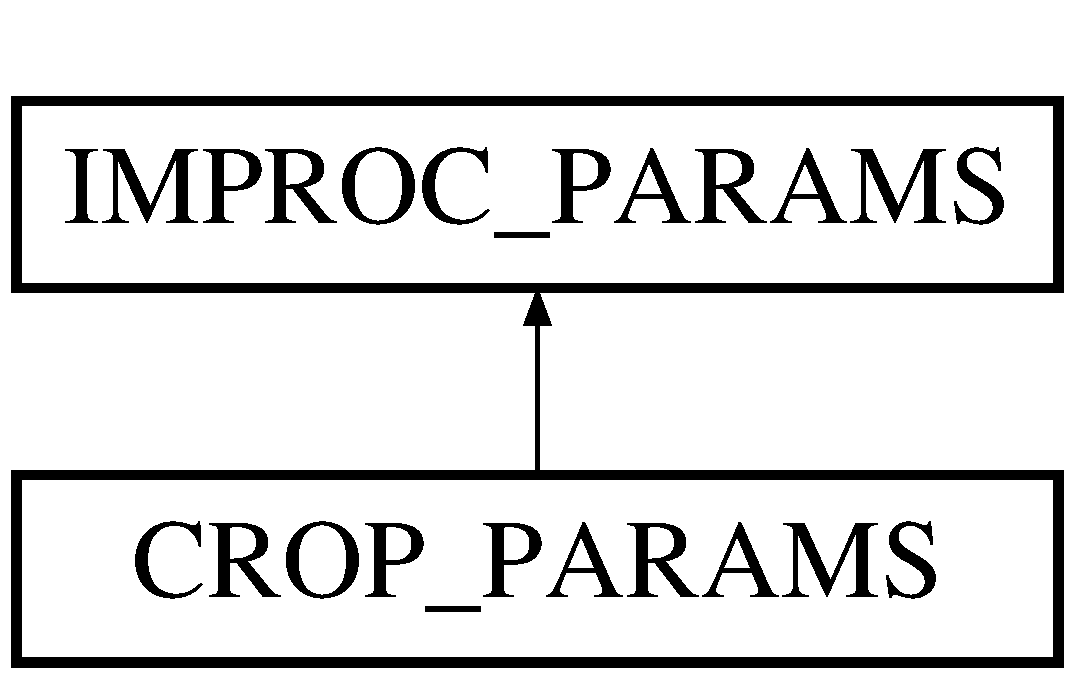
\includegraphics[height=2.000000cm]{struct_c_r_o_p___p_a_r_a_m_s}
\end{center}
\end{figure}
\subsection*{Public Attributes}
\begin{DoxyCompactItemize}
\item 
\hypertarget{struct_c_r_o_p___p_a_r_a_m_s_a2c691b79b6a12648ad3468bbb594a373}{int {\bfseries par1} = 0}\label{struct_c_r_o_p___p_a_r_a_m_s_a2c691b79b6a12648ad3468bbb594a373}

\item 
\hypertarget{struct_c_r_o_p___p_a_r_a_m_s_afe374993a90303a45b0db511388c2d58}{float {\bfseries par2}}\label{struct_c_r_o_p___p_a_r_a_m_s_afe374993a90303a45b0db511388c2d58}

\end{DoxyCompactItemize}


The documentation for this struct was generated from the following file\+:\begin{DoxyCompactItemize}
\item 
Im\+\_\+processing.\+hpp\end{DoxyCompactItemize}

\hypertarget{struct_e_x_t_r_a_c_t_o_r___d_a_t_a}{\section{E\+X\+T\+R\+A\+C\+T\+O\+R\+\_\+\+D\+A\+T\+A Struct Reference}
\label{struct_e_x_t_r_a_c_t_o_r___d_a_t_a}\index{E\+X\+T\+R\+A\+C\+T\+O\+R\+\_\+\+D\+A\+T\+A@{E\+X\+T\+R\+A\+C\+T\+O\+R\+\_\+\+D\+A\+T\+A}}
}
\subsection*{Public Attributes}
\begin{DoxyCompactItemize}
\item 
\hypertarget{struct_e_x_t_r_a_c_t_o_r___d_a_t_a_ab6fa793ad8bbc0b879b000abb75b9747}{enum\+Descriptors {\bfseries tipo}}\label{struct_e_x_t_r_a_c_t_o_r___d_a_t_a_ab6fa793ad8bbc0b879b000abb75b9747}

\item 
\hypertarget{struct_e_x_t_r_a_c_t_o_r___d_a_t_a_a65f3e7ba03a1182700f4052402035340}{\hyperlink{struct_e_x_t_r_a_c_t_o_r___p_a_r_a_m_s}{E\+X\+T\+R\+A\+C\+T\+O\+R\+\_\+\+P\+A\+R\+A\+M\+S} {\bfseries parametros}}\label{struct_e_x_t_r_a_c_t_o_r___d_a_t_a_a65f3e7ba03a1182700f4052402035340}

\end{DoxyCompactItemize}


The documentation for this struct was generated from the following file\+:\begin{DoxyCompactItemize}
\item 
Ftr\+\_\+extractor.\+hpp\end{DoxyCompactItemize}

\hypertarget{struct_e_x_t_r_a_c_t_o_r___p_a_r_a_m_s}{\section{E\+X\+T\+R\+A\+C\+T\+O\+R\+\_\+\+P\+A\+R\+A\+M\+S Struct Reference}
\label{struct_e_x_t_r_a_c_t_o_r___p_a_r_a_m_s}\index{E\+X\+T\+R\+A\+C\+T\+O\+R\+\_\+\+P\+A\+R\+A\+M\+S@{E\+X\+T\+R\+A\+C\+T\+O\+R\+\_\+\+P\+A\+R\+A\+M\+S}}
}
Inheritance diagram for E\+X\+T\+R\+A\+C\+T\+O\+R\+\_\+\+P\+A\+R\+A\+M\+S\+:\begin{figure}[H]
\begin{center}
\leavevmode
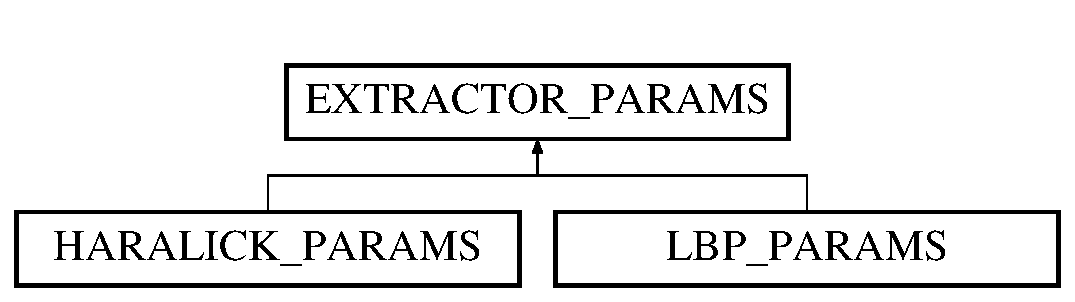
\includegraphics[height=2.000000cm]{struct_e_x_t_r_a_c_t_o_r___p_a_r_a_m_s}
\end{center}
\end{figure}


The documentation for this struct was generated from the following file\+:\begin{DoxyCompactItemize}
\item 
Ftr\+\_\+extractor.\+hpp\end{DoxyCompactItemize}

\hypertarget{class_ftr__extractor}{\section{Ftr\+\_\+extractor Class Reference}
\label{class_ftr__extractor}\index{Ftr\+\_\+extractor@{Ftr\+\_\+extractor}}
}
Inheritance diagram for Ftr\+\_\+extractor\+:\begin{figure}[H]
\begin{center}
\leavevmode
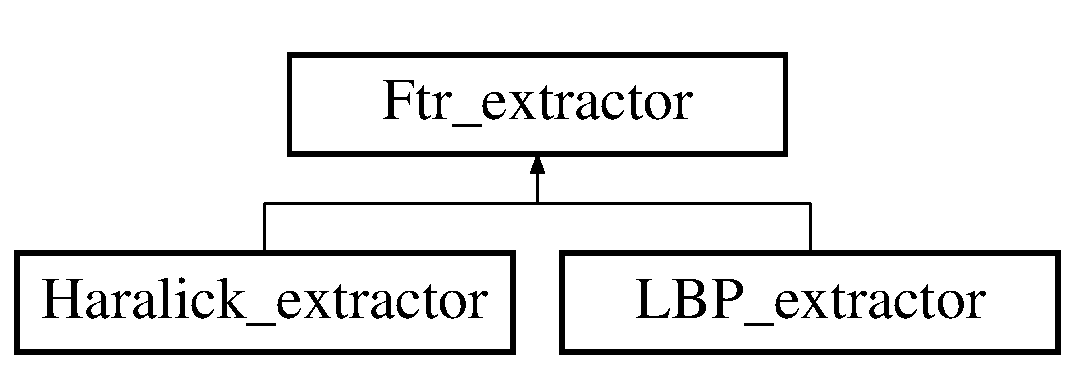
\includegraphics[height=2.000000cm]{class_ftr__extractor}
\end{center}
\end{figure}
\subsection*{Public Member Functions}
\begin{DoxyCompactItemize}
\item 
\hypertarget{class_ftr__extractor_ad7cc765a1f09452f5257bfe84ec5f9b0}{virtual int $\ast$ {\bfseries calculate\+\_\+vector} (int $\ast$n)=0}\label{class_ftr__extractor_ad7cc765a1f09452f5257bfe84ec5f9b0}

\end{DoxyCompactItemize}


The documentation for this class was generated from the following file\+:\begin{DoxyCompactItemize}
\item 
Ftr\+\_\+extractor.\+hpp\end{DoxyCompactItemize}

\hypertarget{class_haralick__extractor}{\section{Haralick\+\_\+extractor Class Reference}
\label{class_haralick__extractor}\index{Haralick\+\_\+extractor@{Haralick\+\_\+extractor}}
}
Inheritance diagram for Haralick\+\_\+extractor\+:\begin{figure}[H]
\begin{center}
\leavevmode
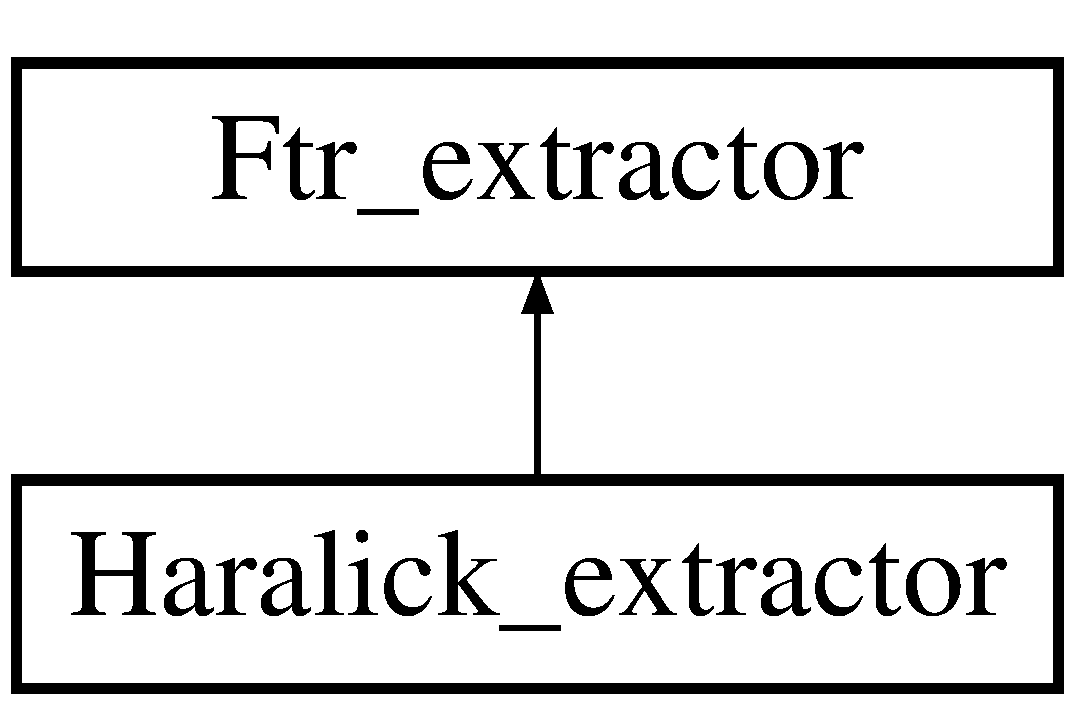
\includegraphics[height=2.000000cm]{class_haralick__extractor}
\end{center}
\end{figure}
\subsection*{Public Member Functions}
\begin{DoxyCompactItemize}
\item 
\hypertarget{class_haralick__extractor_a11fcc043c9abe6d00ae337ea7f5048f9}{int $\ast$ {\bfseries calculate\+\_\+vector} (int $\ast$n)}\label{class_haralick__extractor_a11fcc043c9abe6d00ae337ea7f5048f9}

\end{DoxyCompactItemize}


The documentation for this class was generated from the following files\+:\begin{DoxyCompactItemize}
\item 
Ftr\+\_\+extractor.\+hpp\item 
Ftr\+\_\+extractor.\+cpp\end{DoxyCompactItemize}

\hypertarget{struct_h_a_r_a_l_i_c_k___p_a_r_a_m_s}{\section{H\+A\+R\+A\+L\+I\+C\+K\+\_\+\+P\+A\+R\+A\+M\+S Struct Reference}
\label{struct_h_a_r_a_l_i_c_k___p_a_r_a_m_s}\index{H\+A\+R\+A\+L\+I\+C\+K\+\_\+\+P\+A\+R\+A\+M\+S@{H\+A\+R\+A\+L\+I\+C\+K\+\_\+\+P\+A\+R\+A\+M\+S}}
}


The documentation for this struct was generated from the following file\+:\begin{DoxyCompactItemize}
\item 
Ftr\+\_\+extractor.\+hpp\end{DoxyCompactItemize}

\hypertarget{class_im__processing}{\section{Im\+\_\+processing Class Reference}
\label{class_im__processing}\index{Im\+\_\+processing@{Im\+\_\+processing}}
}
Inheritance diagram for Im\+\_\+processing\+:\begin{figure}[H]
\begin{center}
\leavevmode
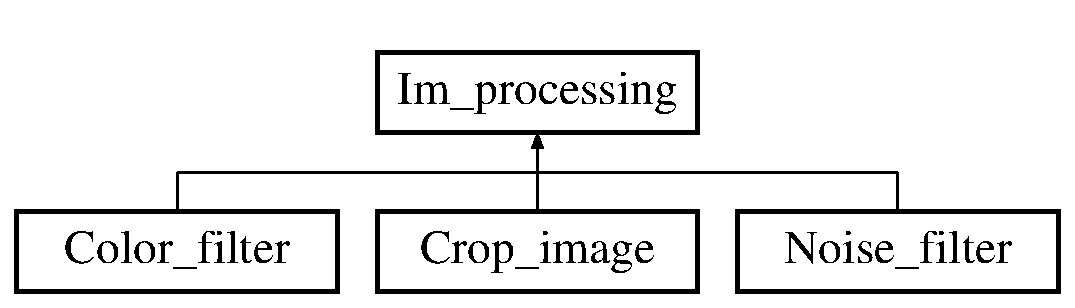
\includegraphics[height=2.000000cm]{class_im__processing}
\end{center}
\end{figure}
\subsection*{Public Member Functions}
\begin{DoxyCompactItemize}
\item 
\hypertarget{class_im__processing_a7219f34f46e683ef214fbc26a0cc3311}{virtual void {\bfseries apply} (int $\ast$n)=0}\label{class_im__processing_a7219f34f46e683ef214fbc26a0cc3311}

\end{DoxyCompactItemize}


The documentation for this class was generated from the following file\+:\begin{DoxyCompactItemize}
\item 
Im\+\_\+processing.\+hpp\end{DoxyCompactItemize}

\hypertarget{struct_i_m_p_r_o_c___d_a_t_a}{\section{I\+M\+P\+R\+O\+C\+\_\+\+D\+A\+T\+A Struct Reference}
\label{struct_i_m_p_r_o_c___d_a_t_a}\index{I\+M\+P\+R\+O\+C\+\_\+\+D\+A\+T\+A@{I\+M\+P\+R\+O\+C\+\_\+\+D\+A\+T\+A}}
}
\subsection*{Public Attributes}
\begin{DoxyCompactItemize}
\item 
\hypertarget{struct_i_m_p_r_o_c___d_a_t_a_a6a0be95cf91d45344249b244a1f99a0a}{enum\+Im\+Processing {\bfseries type}}\label{struct_i_m_p_r_o_c___d_a_t_a_a6a0be95cf91d45344249b244a1f99a0a}

\item 
\hypertarget{struct_i_m_p_r_o_c___d_a_t_a_a46380fc6a06f8e95f6a19c2e541ef9c8}{\hyperlink{struct_i_m_p_r_o_c___p_a_r_a_m_s}{I\+M\+P\+R\+O\+C\+\_\+\+P\+A\+R\+A\+M\+S} {\bfseries parametros}}\label{struct_i_m_p_r_o_c___d_a_t_a_a46380fc6a06f8e95f6a19c2e541ef9c8}

\end{DoxyCompactItemize}


The documentation for this struct was generated from the following file\+:\begin{DoxyCompactItemize}
\item 
Im\+\_\+processing.\+hpp\end{DoxyCompactItemize}

\hypertarget{struct_i_m_p_r_o_c___p_a_r_a_m_s}{\section{I\+M\+P\+R\+O\+C\+\_\+\+P\+A\+R\+A\+M\+S Struct Reference}
\label{struct_i_m_p_r_o_c___p_a_r_a_m_s}\index{I\+M\+P\+R\+O\+C\+\_\+\+P\+A\+R\+A\+M\+S@{I\+M\+P\+R\+O\+C\+\_\+\+P\+A\+R\+A\+M\+S}}
}
Inheritance diagram for I\+M\+P\+R\+O\+C\+\_\+\+P\+A\+R\+A\+M\+S\+:\begin{figure}[H]
\begin{center}
\leavevmode
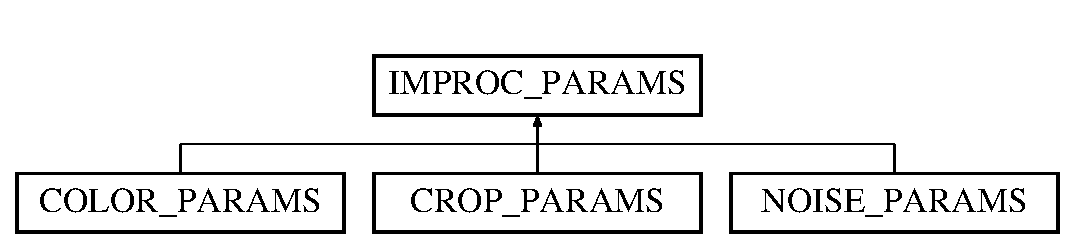
\includegraphics[height=2.000000cm]{struct_i_m_p_r_o_c___p_a_r_a_m_s}
\end{center}
\end{figure}
\subsection*{Public Attributes}
\begin{DoxyCompactItemize}
\item 
\hypertarget{struct_i_m_p_r_o_c___p_a_r_a_m_s_a9c9573a9ddf01e2cb8dcee79d581cc7f}{enum\+Im\+Processing {\bfseries type}}\label{struct_i_m_p_r_o_c___p_a_r_a_m_s_a9c9573a9ddf01e2cb8dcee79d581cc7f}

\end{DoxyCompactItemize}


The documentation for this struct was generated from the following file\+:\begin{DoxyCompactItemize}
\item 
Im\+\_\+processing.\+hpp\end{DoxyCompactItemize}

\hypertarget{class_k_n_n___model}{\section{K\+N\+N\+\_\+\+Model Class Reference}
\label{class_k_n_n___model}\index{K\+N\+N\+\_\+\+Model@{K\+N\+N\+\_\+\+Model}}
}
Inheritance diagram for K\+N\+N\+\_\+\+Model\+:\begin{figure}[H]
\begin{center}
\leavevmode
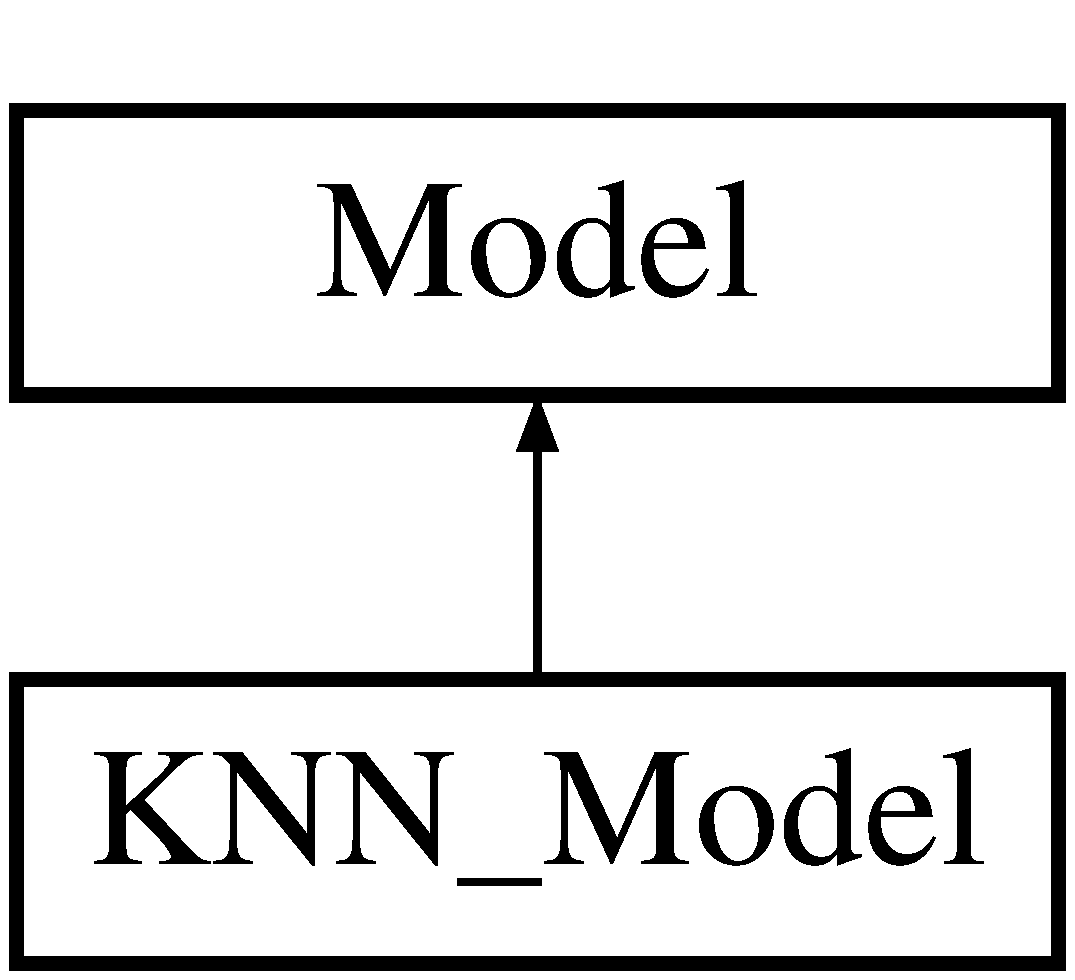
\includegraphics[height=2.000000cm]{class_k_n_n___model}
\end{center}
\end{figure}
\subsection*{Public Member Functions}
\begin{DoxyCompactItemize}
\item 
\hypertarget{class_k_n_n___model_a5ab1a3f5080368e42b9961fa6aa9f23e}{{\bfseries K\+N\+N\+\_\+\+Model} (cv\+::\+Mat $\ast$params)}\label{class_k_n_n___model_a5ab1a3f5080368e42b9961fa6aa9f23e}

\item 
\hypertarget{class_k_n_n___model_adafb1d8355243cd343d318470eefca66}{cv\+::\+Mat {\bfseries classify} (cv\+::\+Input\+Array vetor\+\_\+descritor)}\label{class_k_n_n___model_adafb1d8355243cd343d318470eefca66}

\item 
\hypertarget{class_k_n_n___model_a0b5ed5f2754161b1efde171939620fc1}{void {\bfseries train} (cv\+::\+Mat \&samples, cv\+::\+Mat \&responses)}\label{class_k_n_n___model_a0b5ed5f2754161b1efde171939620fc1}

\end{DoxyCompactItemize}
\subsection*{Additional Inherited Members}


The documentation for this class was generated from the following files\+:\begin{DoxyCompactItemize}
\item 
Model.\+hpp\item 
Model.\+cpp\end{DoxyCompactItemize}

\hypertarget{class_k_n_n__trainer}{\section{K\+N\+N\+\_\+trainer Class Reference}
\label{class_k_n_n__trainer}\index{K\+N\+N\+\_\+trainer@{K\+N\+N\+\_\+trainer}}
}
Inheritance diagram for K\+N\+N\+\_\+trainer\+:\begin{figure}[H]
\begin{center}
\leavevmode
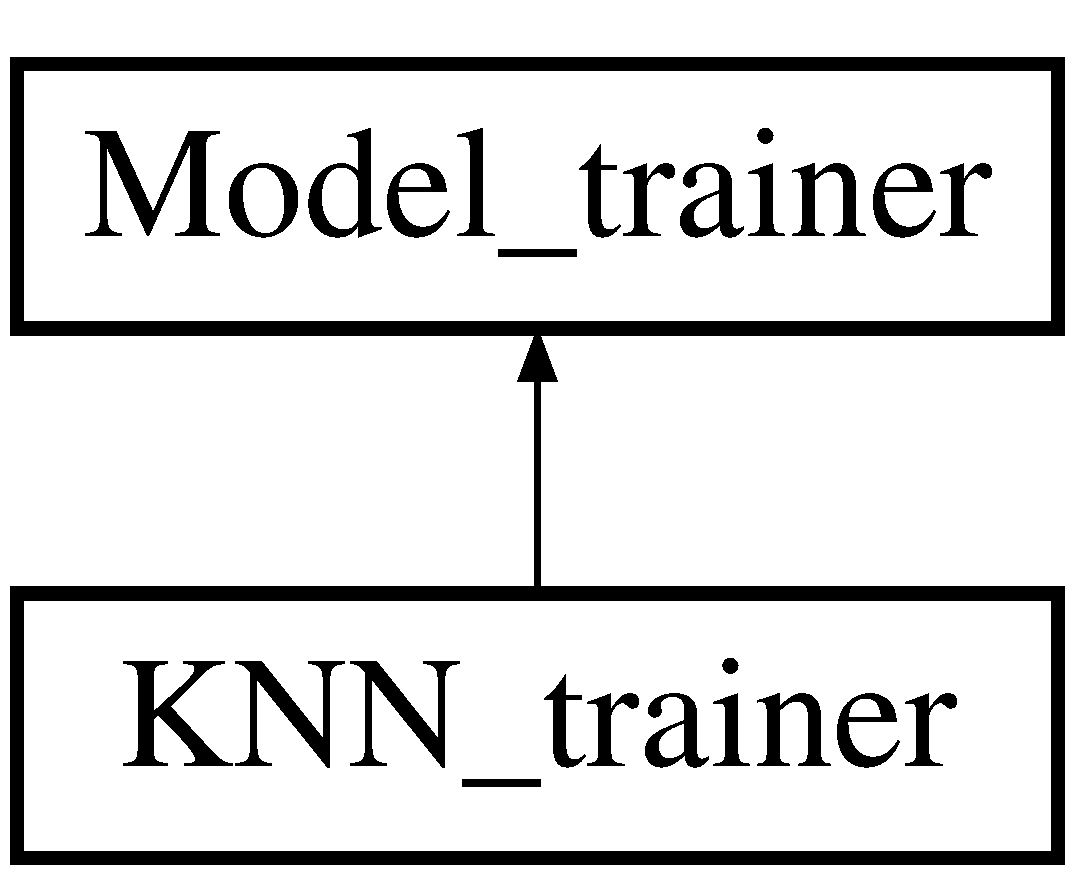
\includegraphics[height=2.000000cm]{class_k_n_n__trainer}
\end{center}
\end{figure}
\subsection*{Additional Inherited Members}


The documentation for this class was generated from the following files\+:\begin{DoxyCompactItemize}
\item 
Model\+\_\+trainer.\+hpp\item 
Model\+\_\+trainer.\+cpp\end{DoxyCompactItemize}

\hypertarget{class_l_b_p__extractor}{\section{L\+B\+P\+\_\+extractor Class Reference}
\label{class_l_b_p__extractor}\index{L\+B\+P\+\_\+extractor@{L\+B\+P\+\_\+extractor}}
}
Inheritance diagram for L\+B\+P\+\_\+extractor\+:\begin{figure}[H]
\begin{center}
\leavevmode
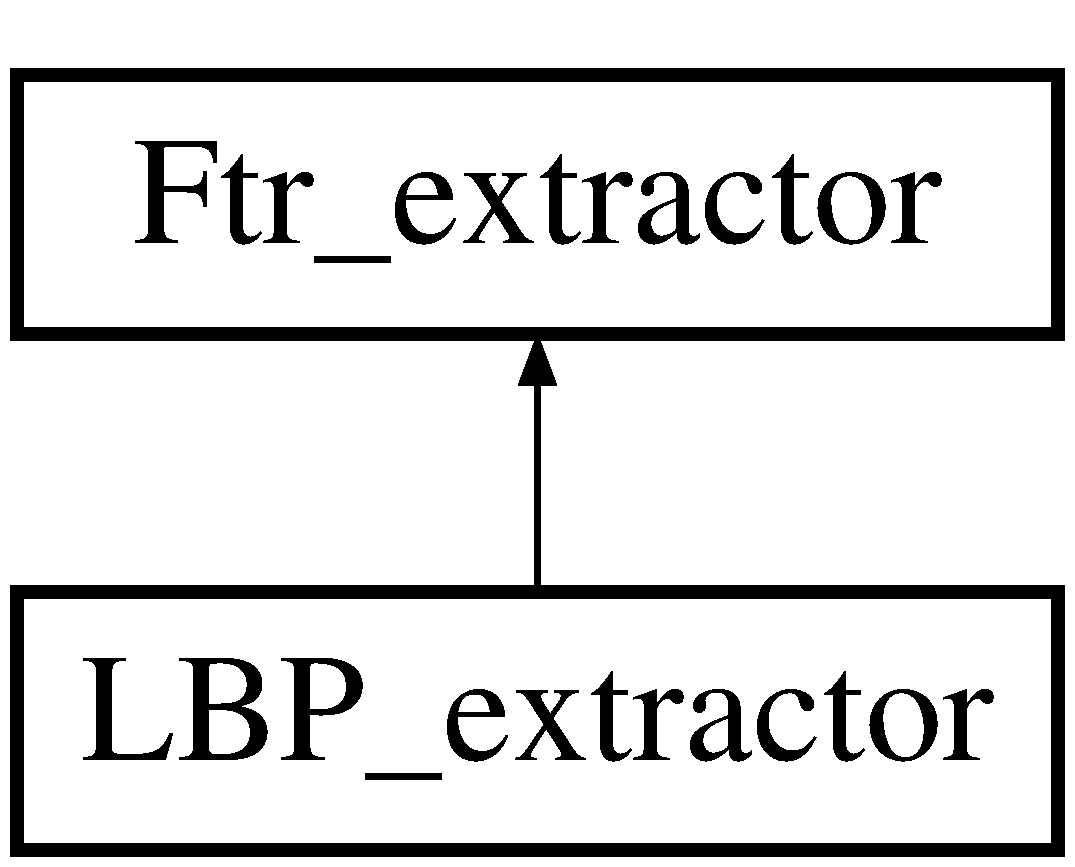
\includegraphics[height=2.000000cm]{class_l_b_p__extractor}
\end{center}
\end{figure}
\subsection*{Public Member Functions}
\begin{DoxyCompactItemize}
\item 
\hypertarget{class_l_b_p__extractor_ad666d4716122f524b416fc3d26669f64}{cv\+::\+Mat $\ast$ {\bfseries calculate\+\_\+vector} (int $\ast$n)}\label{class_l_b_p__extractor_ad666d4716122f524b416fc3d26669f64}

\end{DoxyCompactItemize}


The documentation for this class was generated from the following files\+:\begin{DoxyCompactItemize}
\item 
Ftr\+\_\+extractor.\+hpp\item 
Ftr\+\_\+extractor.\+cpp\end{DoxyCompactItemize}

\hypertarget{struct_l_b_p___p_a_r_a_m_s}{\section{L\+B\+P\+\_\+\+P\+A\+R\+A\+M\+S Struct Reference}
\label{struct_l_b_p___p_a_r_a_m_s}\index{L\+B\+P\+\_\+\+P\+A\+R\+A\+M\+S@{L\+B\+P\+\_\+\+P\+A\+R\+A\+M\+S}}
}


The documentation for this struct was generated from the following file\+:\begin{DoxyCompactItemize}
\item 
Ftr\+\_\+extractor.\+hpp\end{DoxyCompactItemize}

\hypertarget{class_m_l_p___model}{\section{M\+L\+P\+\_\+\+Model Class Reference}
\label{class_m_l_p___model}\index{M\+L\+P\+\_\+\+Model@{M\+L\+P\+\_\+\+Model}}
}
Inheritance diagram for M\+L\+P\+\_\+\+Model\+:\begin{figure}[H]
\begin{center}
\leavevmode
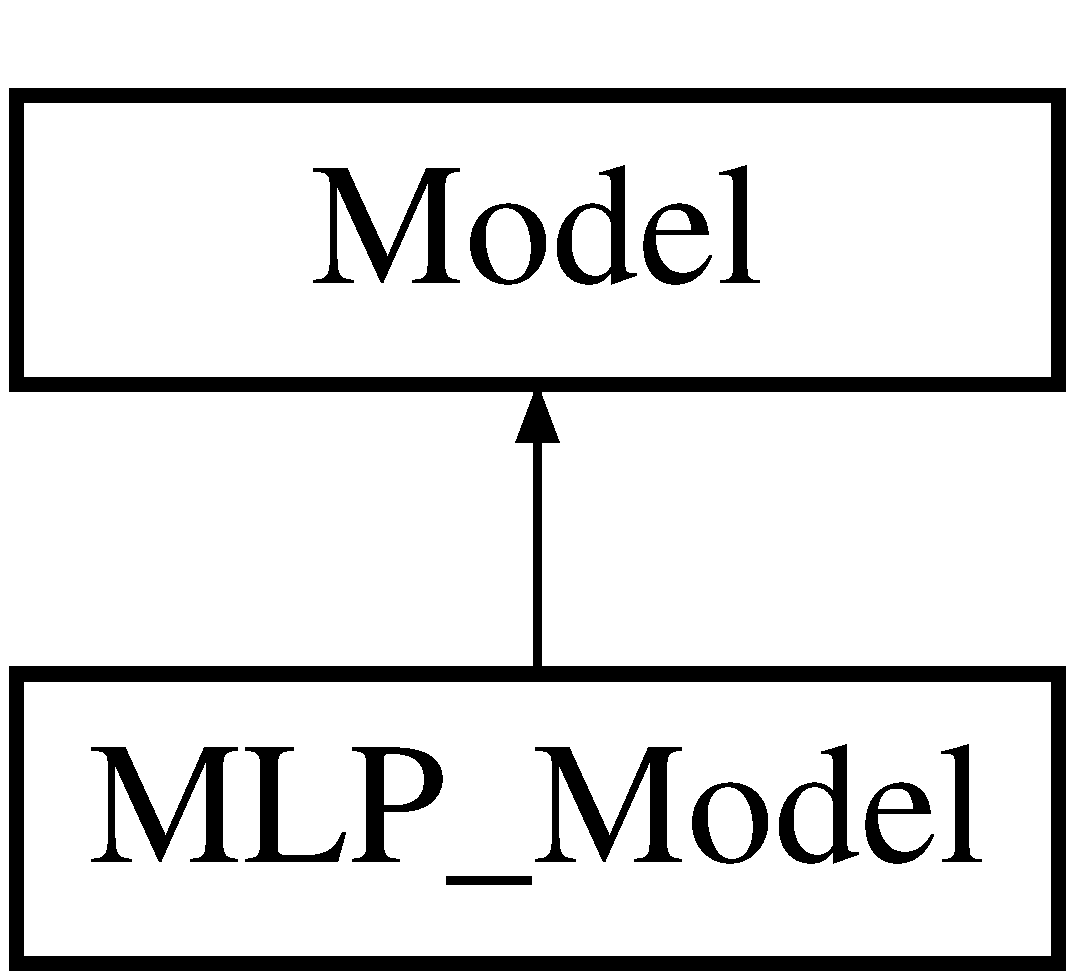
\includegraphics[height=2.000000cm]{class_m_l_p___model}
\end{center}
\end{figure}
\subsection*{Public Member Functions}
\begin{DoxyCompactItemize}
\item 
\hypertarget{class_m_l_p___model_aad376359624227d53d9a235b4e3d1521}{{\bfseries M\+L\+P\+\_\+\+Model} (cv\+::\+Mat $\ast$params)}\label{class_m_l_p___model_aad376359624227d53d9a235b4e3d1521}

\item 
\hypertarget{class_m_l_p___model_a2c6a9b507afa9a8988f2f478210ff47a}{cv\+::\+Mat {\bfseries classify} (cv\+::\+Input\+Array vetor\+\_\+descritor)}\label{class_m_l_p___model_a2c6a9b507afa9a8988f2f478210ff47a}

\item 
\hypertarget{class_m_l_p___model_ae9223d97c1fc30970eb0addfec150a04}{void {\bfseries train} (cv\+::\+Mat \&samples, cv\+::\+Mat \&responses)}\label{class_m_l_p___model_ae9223d97c1fc30970eb0addfec150a04}

\end{DoxyCompactItemize}
\subsection*{Additional Inherited Members}


The documentation for this class was generated from the following files\+:\begin{DoxyCompactItemize}
\item 
Model.\+hpp\item 
Model.\+cpp\end{DoxyCompactItemize}

\hypertarget{class_m_l_p__trainer}{\section{M\+L\+P\+\_\+trainer Class Reference}
\label{class_m_l_p__trainer}\index{M\+L\+P\+\_\+trainer@{M\+L\+P\+\_\+trainer}}
}
Inheritance diagram for M\+L\+P\+\_\+trainer\+:\begin{figure}[H]
\begin{center}
\leavevmode
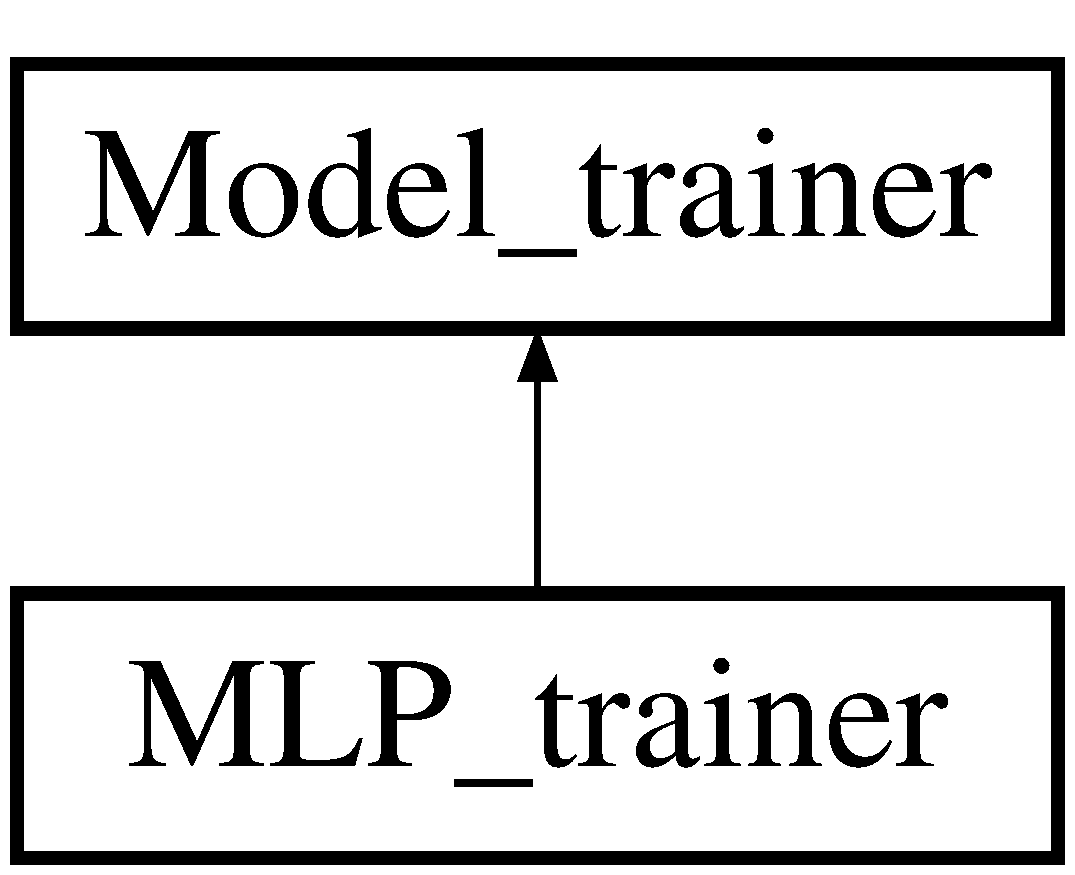
\includegraphics[height=2.000000cm]{class_m_l_p__trainer}
\end{center}
\end{figure}
\subsection*{Additional Inherited Members}


The documentation for this class was generated from the following files\+:\begin{DoxyCompactItemize}
\item 
Model\+\_\+trainer.\+hpp\item 
Model\+\_\+trainer.\+cpp\end{DoxyCompactItemize}

\hypertarget{class_model}{\section{Model Class Reference}
\label{class_model}\index{Model@{Model}}
}
Inheritance diagram for Model\+:\begin{figure}[H]
\begin{center}
\leavevmode
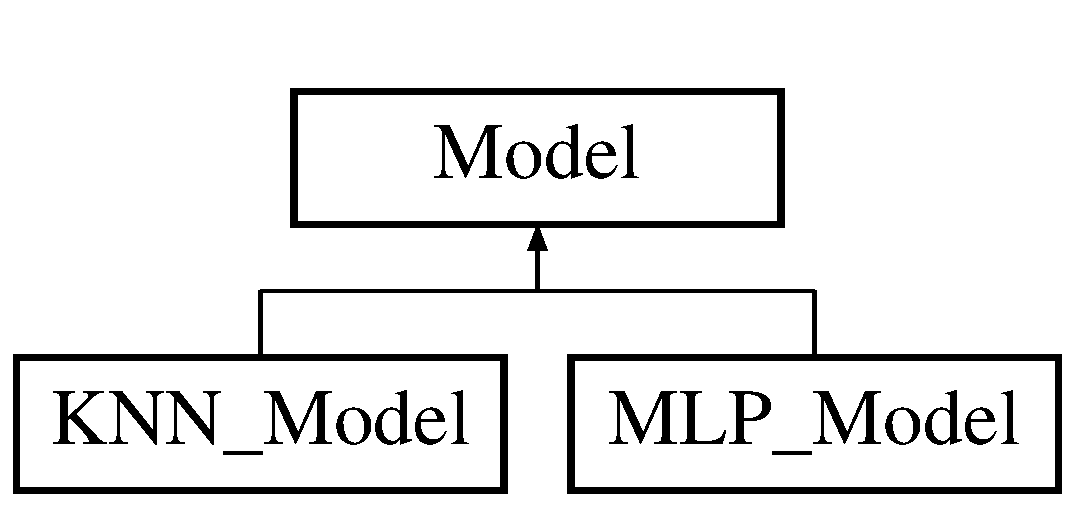
\includegraphics[height=2.000000cm]{class_model}
\end{center}
\end{figure}
\subsection*{Public Member Functions}
\begin{DoxyCompactItemize}
\item 
\hypertarget{class_model_a244b8fc6152e86e20cb581edeef7dac3}{virtual float {\bfseries classify} (Mat $\ast$vetor\+\_\+descritor)=0}\label{class_model_a244b8fc6152e86e20cb581edeef7dac3}

\end{DoxyCompactItemize}


The documentation for this class was generated from the following file\+:\begin{DoxyCompactItemize}
\item 
Model.\+hpp\end{DoxyCompactItemize}

\hypertarget{class_model__trainer}{\section{Model\+\_\+trainer Class Reference}
\label{class_model__trainer}\index{Model\+\_\+trainer@{Model\+\_\+trainer}}
}
\subsection*{Public Member Functions}
\begin{DoxyCompactItemize}
\item 
\hypertarget{class_model__trainer_a1255f492c38a0386dffc299264713ebe}{virtual void {\bfseries train} ()=0}\label{class_model__trainer_a1255f492c38a0386dffc299264713ebe}

\item 
\hypertarget{class_model__trainer_ae8e4dc1b16703f078819b43b5ae89a20}{float {\bfseries evaluate} ()}\label{class_model__trainer_ae8e4dc1b16703f078819b43b5ae89a20}

\end{DoxyCompactItemize}


The documentation for this class was generated from the following file\+:\begin{DoxyCompactItemize}
\item 
Model\+\_\+trainer.\+hpp\end{DoxyCompactItemize}

\hypertarget{class_noise__filter}{\section{Noise\+\_\+filter Class Reference}
\label{class_noise__filter}\index{Noise\+\_\+filter@{Noise\+\_\+filter}}
}
Inheritance diagram for Noise\+\_\+filter\+:\begin{figure}[H]
\begin{center}
\leavevmode
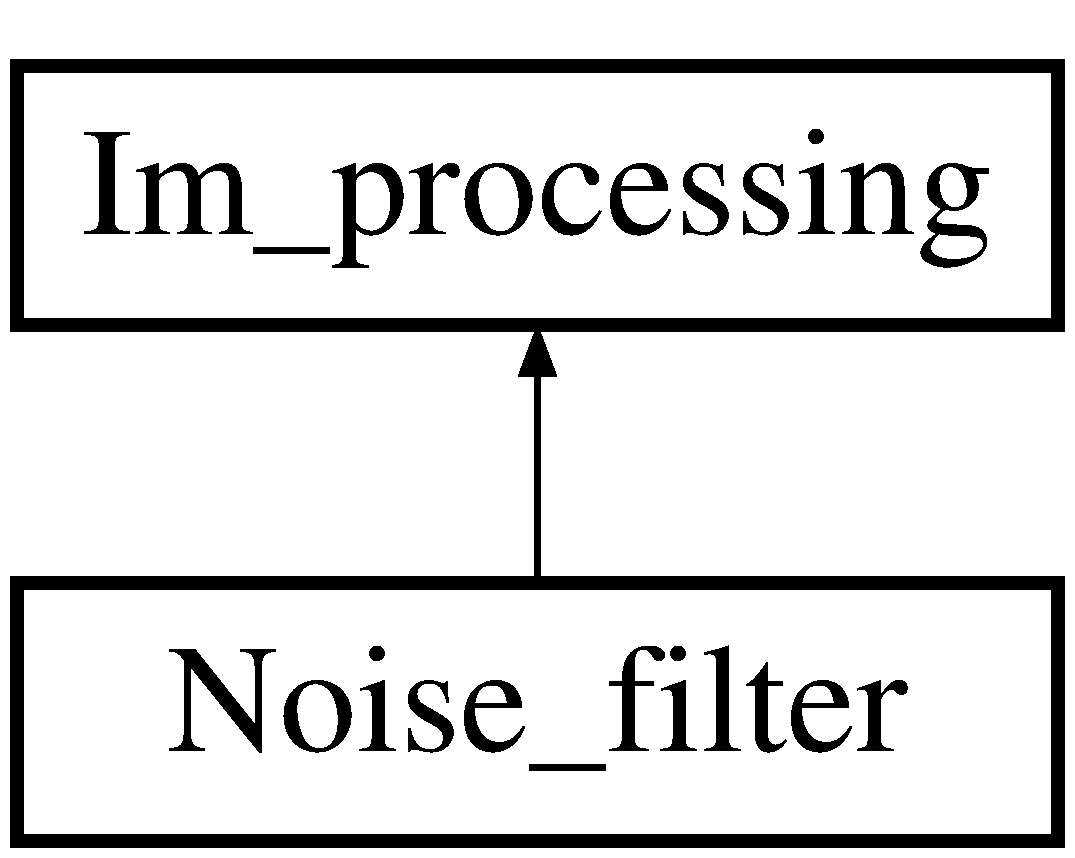
\includegraphics[height=2.000000cm]{class_noise__filter}
\end{center}
\end{figure}
\subsection*{Public Member Functions}
\begin{DoxyCompactItemize}
\item 
\hypertarget{class_noise__filter_aeb680eda9dc62351d67c0a89a26bc3f4}{void {\bfseries apply} (int $\ast$n)}\label{class_noise__filter_aeb680eda9dc62351d67c0a89a26bc3f4}

\end{DoxyCompactItemize}


The documentation for this class was generated from the following files\+:\begin{DoxyCompactItemize}
\item 
Im\+\_\+processing.\+hpp\item 
Im\+\_\+processing.\+cpp\end{DoxyCompactItemize}

\hypertarget{struct_n_o_i_s_e___p_a_r_a_m_s}{\section{N\+O\+I\+S\+E\+\_\+\+P\+A\+R\+A\+M\+S Struct Reference}
\label{struct_n_o_i_s_e___p_a_r_a_m_s}\index{N\+O\+I\+S\+E\+\_\+\+P\+A\+R\+A\+M\+S@{N\+O\+I\+S\+E\+\_\+\+P\+A\+R\+A\+M\+S}}
}
Inheritance diagram for N\+O\+I\+S\+E\+\_\+\+P\+A\+R\+A\+M\+S\+:\begin{figure}[H]
\begin{center}
\leavevmode
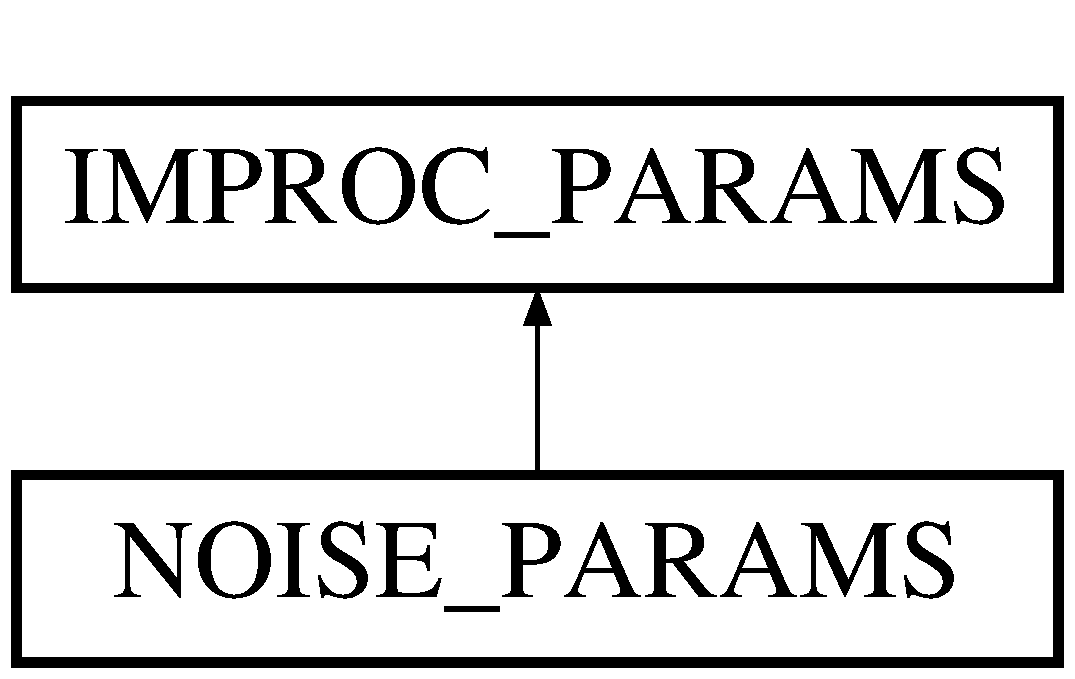
\includegraphics[height=2.000000cm]{struct_n_o_i_s_e___p_a_r_a_m_s}
\end{center}
\end{figure}


The documentation for this struct was generated from the following file\+:\begin{DoxyCompactItemize}
\item 
Im\+\_\+processing.\+hpp\end{DoxyCompactItemize}

%--- End generated contents ---

% Index
\newpage
\phantomsection
\addcontentsline{toc}{chapter}{Index}
\printindex

\end{document}
